\documentclass[a4paper]{article}
\usepackage[utf8]{inputenc}
\usepackage[english]{babel}
\usepackage{amsmath} % per ambienti tipo cases
\usepackage{mathtools}
\usepackage{siunitx}
\usepackage{graphicx} % per includere figure
%\usepackage{subfigure}
\usepackage{booktabs} % per le tabelle
\usepackage{caption}
\usepackage{fancyhdr}
\usepackage{hyperref}
\usepackage[section]{placeins}
\usepackage{microtype}
\usepackage{caption}
\usepackage{subcaption}
\captionsetup[subfigure]{labelfont=rm}
\usepackage{verbatim} %multiline comments
%\usepackage[backend=biber, style=numeric, safeinputenc, sorting=none]{biblatex}
%\addbibresource{source.bib}	% uncomment for bibliography



%opening
\title{}
\author{}

\pagestyle{fancy}
\lhead{Musical Acoustics}
\chead{HL1}
\rhead{10743504, 10751919}
\newcommand{\Rarrow}{\mbox{\Large$\Rightarrow$}}

\begin{document}

\begin{titlepage}	
	\newcommand{\HRule}{\rule{\linewidth}{0.5mm}} % Defines a new command for horizontal lines, change thickness here
	
	\center % Centre everything on the page
	
	%------------------------------------------------
	%	Headings
	%------------------------------------------------
	
	
\includegraphics[width=.4\textwidth]{Logo_Politecnico_Milano.png}\\[0.4cm]
	\textsc{\LARGE}\\[0.3cm] % Main heading such as the name of your university/college
	
	\textsc{\large MSc. Music and Acoustic Engineering}\\[1cm] % Minor heading such as course title
	
	\textsc{\Large Musical Acoustics - A.Y. 2020/2021}\\[0.5cm] % Major heading such as course name
	
	%------------------------------------------------
	%	Title
	%------------------------------------------------
	
	\HRule\\[0.4cm]
	
	{\huge\bfseries HL1 – Comsol Multiphysics }\\[0.4cm] % Title of your document
	
	\HRule\\[1.5cm]
	
	
	
	{\large\textit{Authors' IDs:}}\\
	10743504, 10751919, % Your name
	%\\ \textsc{Gruppo 11}
	
	%------------------------------------------------
	%	Date
	%------------------------------------------------
	
	\vfill\vfill\vfill % Position the date 3/4 down the remaining page
	
	{\large\today} % Date, change the \today to a set date if you want to be precise
	
	%------------------------------------------------
	%	Logo
	%------------------------------------------------
	
	\vfill\vfill
	%\includegraphics[width=0.2\textwidth]{Politecnico_di_Milano.eps}\\[1cm] % Include a department/university logo - this will require the graphicx package
	
	%----------------------------------------------------------------------------------------
	
	\vfill % Push the date up 1/4 of the remaining page
	
	
\end{titlepage}

\section{Church Bell - 3D Model}
\subsection{Model Design}

\begin{figure}[h]
	\centering
	\begin{subfigure}{0.47\linewidth}
		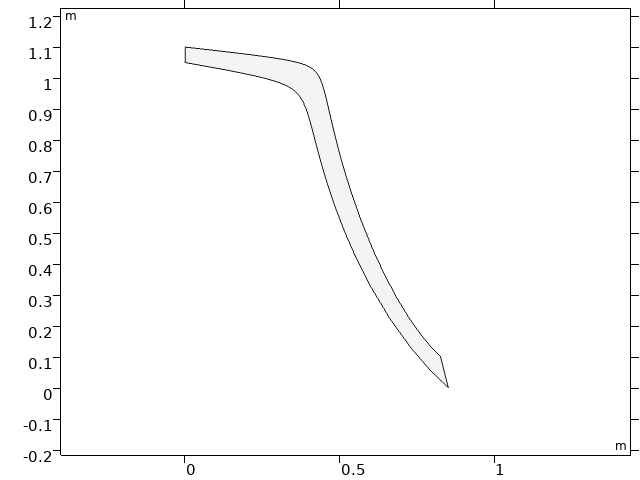
\includegraphics[width=0.9\linewidth]{bell2D.png}
	\end{subfigure}
	~
	\begin{subfigure}{0.47\linewidth}
		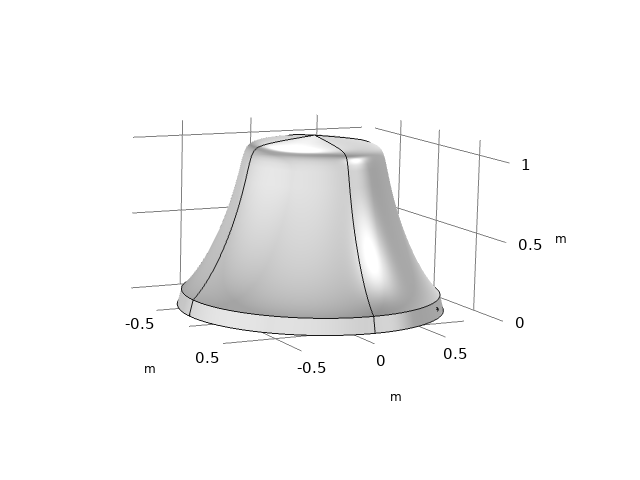
\includegraphics[width=0.9\linewidth]{bell3D.png}
	\end{subfigure}
	\caption{Bézier polygon (on the left) used as a basis for the design and the resulting rotation solid (on the right). }
	\label{fig:shape}
\end{figure}

The modeling of the bell started with the drawing of the 2D shape seen in Fig. \ref{fig:shape}. This is a Bézier polygon, i. e. a closed curve formed by connecting line segments and Bézier curves. In our case we have two cubic Bézier curves connecting two segments, one of which marks the edge of the bell while the other coincides with the intersection of the object with its rotation axis. The actual 3D bell model is indeed obtained by rotating this figure about the $x=0$ line, and it too can be seen in Fig. \ref{fig:shape}.

The way this is done in Comsol is by creating a 3D component, then adding a Work Plane node in its geometry, where the above-mentioned Bézier polygon is drawn, followed by a Revolve node to generate the solid.

The most common material for bellfounding is the aptly named ``bell metal'' which is a kind of bronze with a ratio of copper to tin of roughly 4:1. However, since the bronze alloys available in the Comsol libraries seemed to all have incomplete information regarding their mechanical parameters, we opted for cast iron (from the ``Built-in'' materials library), which is, by the way, another metal that has been historically used for bells, albeit less frequently.

\subsection{Eigenfrequency study}

We performed an eigenfrequency study with free boundary conditions. This meant keeping only the default subnodes in the Solid Mechanics node of our model, of which ``Free 1'' in particular is where the boundary conditions are set. The results are presented in Tab. \ref{tab:freq}.

\begin{table}[h]
	\centering
	$\begin{array}{ll}
		\toprule
		\text{Eigenfrequencies [Hz]} & \text{Angular frequency [rad/s]}\\
				i7.61\times 10^{-5} & i4.78\times 10^{-4} \\
		i1.19\times 10^{-4} &  i7.48\times 10^{-4} \\
		2.03\times 10^{-5} & 1.28\times 10^{-4} \\
		5.19\times 10^{-5} & 3.26\times 10^{-4} \\
		1.1\times 10^{-4} & 6.9\times 10^{-4} \\
		1.29\times 10^{-4} & 8.13\times 10^{-4}  \\
		111.98  &  703.6 \\
		111.98  &  703.6 \\
		262.72 &   1650.7\\ 
		262.72 &   1650.7\\  
		385.48 &   2422.028 \\   
		385.48 &   2422.028 \\ 
		489.14 &  3073.35 \\
     	489.14 &  3073.35 \\
     	509.56  &  3201.69 \\
     	509.56  &  3201.69 \\
		\bottomrule
	\end{array}$
\caption{}
\label{tab:freq}
\end{table}

The first six results are not eigenfrequencies of the system but they refer to the rigid body motion of the bell. Each of them represents one degree of freedom of a tridimensional system in a free configuration. They should have frequency zero but, because of the computational error, are rather very small number. Below these six values, every eigenfrequency shows degeneracy because of the symmetry under axial rotation. Three modeshapes animations can be found in the folder shared with this report: the gifs called "mode 1" and "mode 2" show the lowest pair of degenerate mode, while "mode 9-10" is the eigenshape refered to the last two value of the table. 


\subsection{Time domain study}
We set up a time-domain study to simulate the response of the object to an impulsive force. The impulse was modeled defining a short gaussian pulse in the Definition node of the component. The area where the impulse was applied was defined by taking the intersection between the bell and a cylinder of radius 1 cm with an axis orthogonal to the one of the bell. A force defined with the gaussian pulse was set to be applied to this area by adding a Boundary Load to the physics of the object.

More precisely, all of this was done twice: once on the edge of the bell and once on its side. We report here some snapshots of the results highlighting the displacement of the bell. 

\begin{figure}[h!]
	\centering
	\begin{subfigure}{0.47\textwidth}
		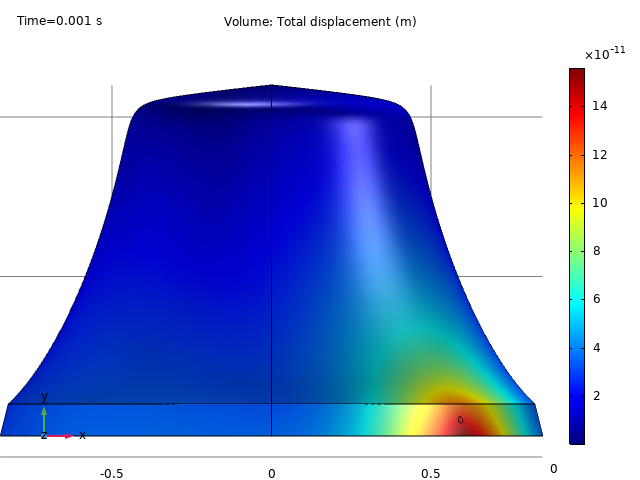
\includegraphics[width=0.8\textwidth]{time domain study edge/initial time.png}
	\end{subfigure}
	~
	\begin{subfigure}{0.47\textwidth}
		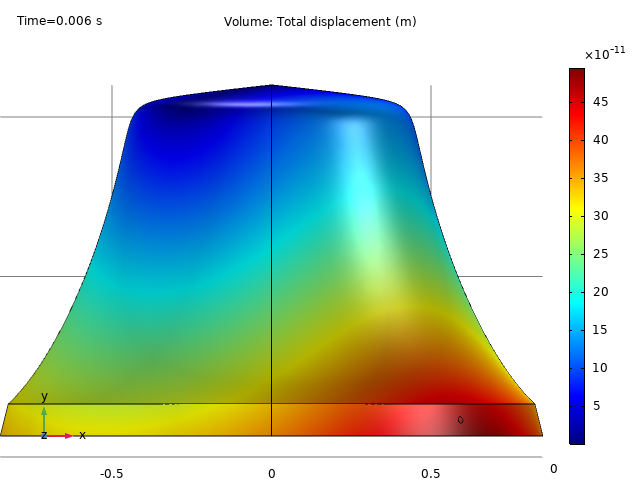
\includegraphics[width=0.8\textwidth]{time domain study edge/initial time 2.png}
	\end{subfigure}

	\begin{subfigure}{0.47\textwidth}
		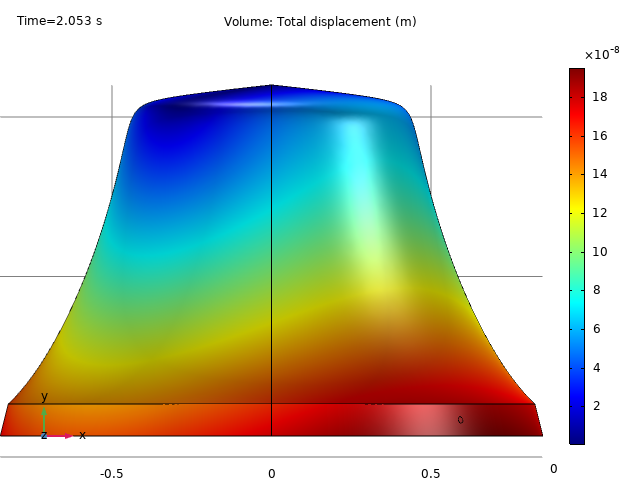
\includegraphics[width=0.8\textwidth]{time domain study edge/middle time.png}
	\end{subfigure}
	~
	\begin{subfigure}{0.47\textwidth}
		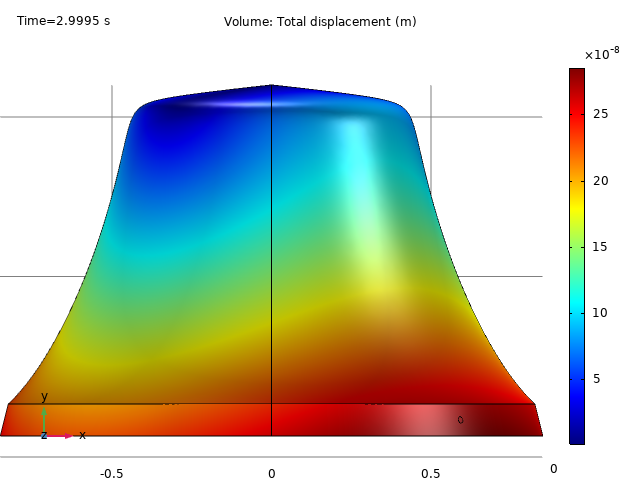
\includegraphics[width=0.8\textwidth]{time domain study edge/final time.png}
	\end{subfigure}
	\caption{Snapshots of the displacement of the surface when the impulse is applied on the \textbf{edge} of the bell.}
	\label{fig:timeEdge}
\end{figure}

\begin{figure}[h!]
	\centering
	\begin{subfigure}{0.47\textwidth}
		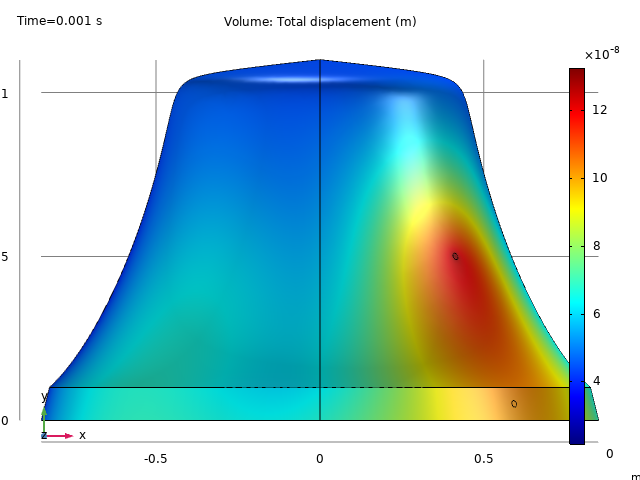
\includegraphics[width=0.8\textwidth]{time domain study side/initial time.png}
	\end{subfigure}
	~
	\begin{subfigure}{0.47\textwidth}
		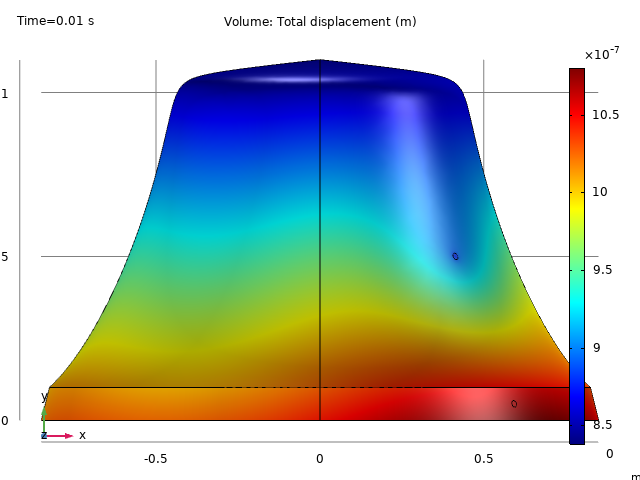
\includegraphics[width=0.8\textwidth]{time domain study side/initial time 2.png}
	\end{subfigure}
	
	\begin{subfigure}{0.47\textwidth}
		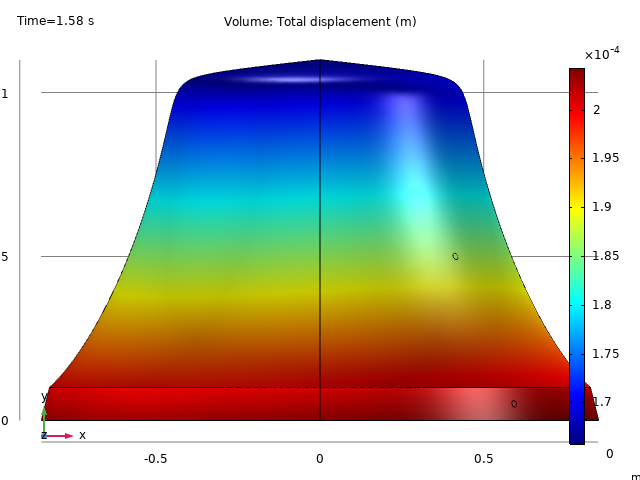
\includegraphics[width=0.8\textwidth]{time domain study side/middle time.png}
	\end{subfigure}
	~
	\begin{subfigure}{0.47\textwidth}
		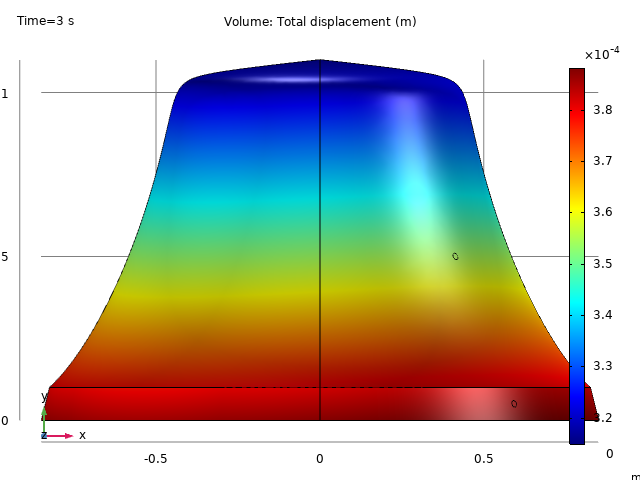
\includegraphics[width=0.8\textwidth]{time domain study side/final time.png}
	\end{subfigure}
	\caption{Snapshots of the displacement of the surface when the impulse is applied on the \textbf{side} of the bell.}
	\label{fig:timeSide}
\end{figure}

\section{Church Bell - 2D Axisymmetric Model}

\begin{figure}[h!]
	\centering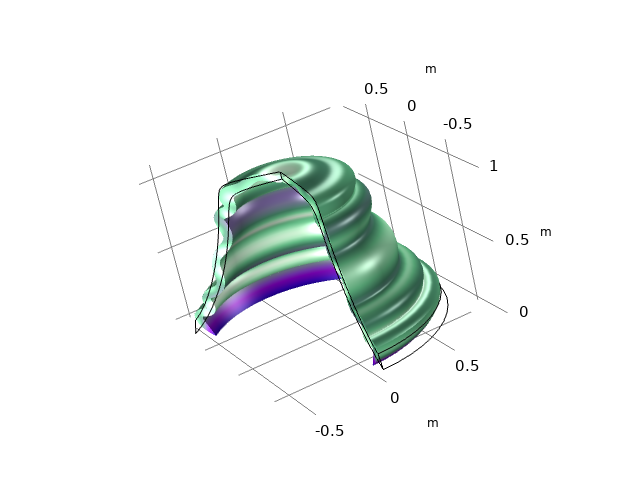
\includegraphics[width=0.75\linewidth]{axisMode.png}
	\caption{Mode shape with axial symmetry.}
	\label{fig:ax}
\end{figure}

In this case we simply imported the same 2D figure as before in the Geometry node of a 2D-axisymmetric component. We then performed an eigenfrequency study much like in the previous case. The eigenfrequencies do not appear to be the same as before. The main reason is that for a 2D-axisymmetric component, studies get carried out on the 2D shape and then the results are extrapolated to the entire object under the assumption that we are only looking for axysimmetric properties. When looking for vibration eigenmodes, this means that we are ignoring the modes that do not exhibit this symmetry, which in our case were all the modes studied previously.

\end{document}